\documentclass{report}
\title{\textbf{\Huge Thermal Power Plants} }
\author{Divya Raj \bullet 1610110123 \\ Himanshu Sharma \bullet 1610110149 \\ Vedansh Gupta \bullet 1610110429}
\date{}

\usepackage[margin=1.4in]{geometry}
\usepackage{graphicx}
\usepackage{float}
\usepackage{amsmath}

\begin{document}
\maketitle
\tableofcontents
\newpage
\renewcommand{\thesection}{\arabic{section}}
\section{Introduction}
Thermal Power Plants as the title infers is the place of mechanism which converts heat energy into electric power. In thermal power plants, the heat energy obtained from combustion of solid fuel (mostly coal) is used to convert water into steam, this steam is at high pressure and temperature. This steam is used to rotate the turbine blade which is connected to the generator. The generator converts the kinetic energy of the turbine impeller into electric energy.
\par Thermal power plants are the largest source of power in India. Thermal energy, which is used to convert heat into electricity is based on three types of heat sources.
\begin{enumerate}
\item{Coal - More than 62 \% demand is met by coal reserves. NTPC and other state level power generation companies are engaged in maintaining and operating thermal power plants.}
\item{Gas - Use Natural Gas.}
\item{Diesel}
\end{enumerate}
A structured thermal power plant is shown below. The diagram has been taken from Wikipedia.

\begin{figure}[H]
\centering 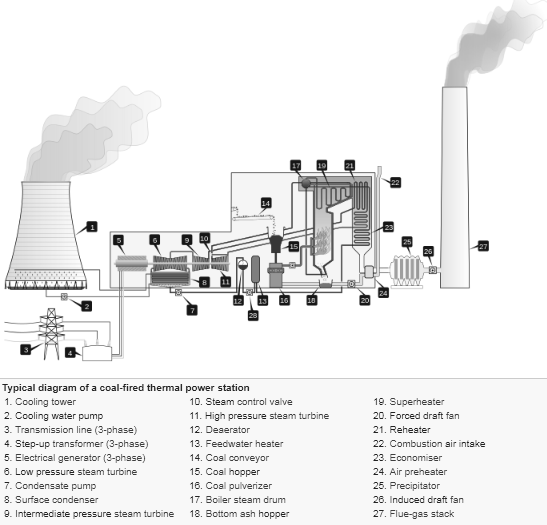
\includegraphics[width=0.9\textwidth]{images/tpp1.png}
\caption{General structure of a Thermal Power Plant}
\end{figure}

\section{Working Components of a Thermal Power Plant}
The plant is a system, and a system needs harmonical contributions of some components. These components in their actual form are discussed below one by one. The work-flow of a thermal power plant is in the following manner. Fuel (which has generally large particle size) is crushed down to smaller particle size. It is then combusted to generate heat. This heat is then transferred to running water which then turns to high pressure steam. Generally, gases from the boiler exhaust are at high temperature and if this heat is not utilized will lead to a large amount of losses resulting in reduced boiler efficiency. So generally this waste heat is recovered by heating either air required for combustion or preheat water before sending it into a boiler. Gases are then allowed to pass through a dust collector or a bag filter to arrest dust particles so as to prevent air pollution before sending it to the atmosphere through a chimney.
\subsection{Fuel Storage Facility}
Fuel is an important resource. Any plant which depends extensively on fuel needs to store it somewhere from where it could be used later on when the supply of fuel from the mine is improper. This is where a fuel storage facility comes into picture. \par In a thermal power plant, the first step in process of power generation is that the fuel is brought to breaker house with the help of belt conveyor, here light dust is separated with the help of rotary machine through the action of gravity. It further goes to the crusher where it is crushed to a size of about 50mm.
\subsection{Water Treatment Facility}
The water that has been converted to steam, is brought to the turbines under high pressure. This steam is used to rotate them. Normal water is taken from the river, and it contains a lot of dirt, suspended particulate matter (SPM), dissolved minerals and dissolved gases such as air etc. If the water fed to the boiler is not treated, it will reduce the life and efficiency of equipment by corroding the surfaces which may lead to overheating of pressure parts and explosions. \par This particulate matter is separated out by adding {\it alum} into the water. Alum coagulates the dirt and increases its density. Then, due to gravity, this coagulated matter settles down in the water which is then removed from it. 

\begin{figure}[H]
\centering 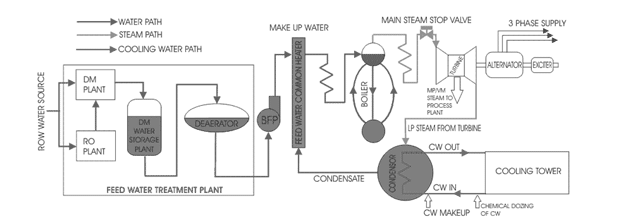
\includegraphics[width=\textwidth]{images/tpp2.png}
\caption{Water treatment}
\end{figure}

\par After gravity separation, water softening is done by ion exchange process. As the hardness comes through the carbonates and bicarbonates of sodium and magnesium, these salts are removed from water anion exchange and cation exchange process. \par Water also contains dissolved oxygen and this leads to corrosion and fouling of boiler tubes and surfaces when it comes in their contact. So removing dissolved oxygen from water is done by adding oxygen scavengers and by using a Deaerator tank. Deaerator tank also acts as a feed water tank to store the feed water. On heating feed water in a deaerator tank decreases the solubility of air in water, thereby removing the dissolved air from the water.
\subsection{Boiler}
A boiler is a high pressure vessel used to generate high pressure steam at saturated temperatures. Water tube boiler consists of a furnace enclosed by the water tubes membrane. The crushed fuel from the crushers is fed into the boiler furnace over the grate. The hot air from the Forced Draft (FD) fan is mixed with the crushed fuel causing combustion of fuel.
\begin{figure}[H]
\centering 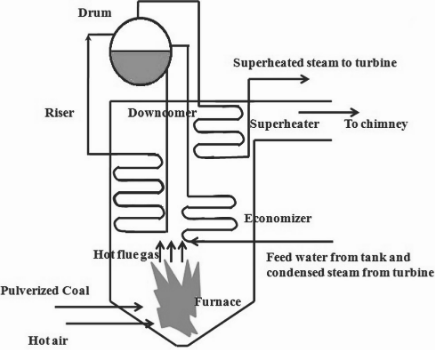
\includegraphics[width=0.6\textwidth]{images/tpp3.png}
\caption{Boiler}
\end{figure}
Combustion of fuel generates a lot of radiation heat which is transferred to water in the membrane tubes. Flue gases generated during combustion travel at high velocity across the convection bank of tubes thereby heating water through convection heat transfer. Hot water is sent to a boiler drum at high pressure through the feed water pump. The boiler tubes which are in contact with low temperature acts as downcomers to circulate the water while the tubes which are in contact with high temperature acts as risers to carry steam. This leads to an effective circulation of water thereby preventing the tubes from getting overheated.

Steam leaving the boiler is at a saturated temperature and pressure but there are a lot of heat losses during its transportation to the turbines. So to increase the quality of steam, steam Superheater is installed in a radiative section of a boiler to increase its temperature and dryness fraction without increasing its pressure as well as to accommodate for the transportation temperature losses.

The exhaust gases leaving the boiler are generally at high temperature and this waste heat is extracted by installing an Economiser or Water Pre heaters to preheat the feed water to the boiler and Air Preheaters to pre-heat the air coming from the Forced Draft Fan required for the combustion of fuel. Installing this equipment help to decrease the flue gas temperature thereby increasing the efficiency.

The flue gases leaving the boiler also contain some ash particles, so to reduce the air pollution, flue gases are allowed to pass through the Dust Collectors and Bag Filters to remove the ash particulates from the flue gases and are sometimes passed through the Wet Scrubbers to decrease the sulfur content from the gases.

The flue gases are drawn through this equipment using an Induced Draft (ID) Fan which is designed for a fixed capacity and head to prevent any back pressure. After the ID fan, flue gases are exhausted off into the atmosphere using a chimney.

\subsection{Turbine}
A turbine is a mechanical device which converts the kinetic and pressure energy of steam into useful work. From the superheater steam goes to the turbine where it expands and loses its kinetic and pressure energy and rotates the turbine blade which in turn rotates the turbine shaft connected to its blades. The shaft then rotates the generator which converts this kinetic energy into electrical energy.

\section{Working process of a Thermal Power Plant}
While we have discussed the different components of a thermal power plant, we still need to know the most efficient process of generating energy from the heat source. Broadly speaking we have this block diagram for a general power plant.
\\
\begin{figure}[H]
\centering 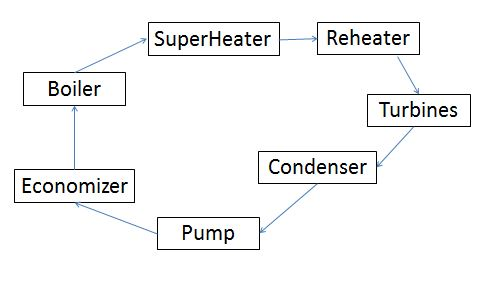
\includegraphics[width=0.6\textwidth]{captures/Capture1.JPG}
\caption{Power Plant}
\end{figure}
\par A pump is needed because boiler is at high pressure and temperature and condenser is at low pressure and temperature. Because of such sudden change from low pressure to high pressure we need it. Turbine converts high pressure steam to low pressure. Hence both turbine and pump are doing same kind of work but doing it in opposite direction. So whatever energy is coming out of the turbine is required to run the pump. This is called a {\it Rankine cycle}. 
\subsection{The temperature-entropy diagram for the Thermal Power Plant}
For fluids we draw a $T-S$ diagram. A $T-S$ diagram for water is shown below. 
\\
\begin{figure}[H]
\centering 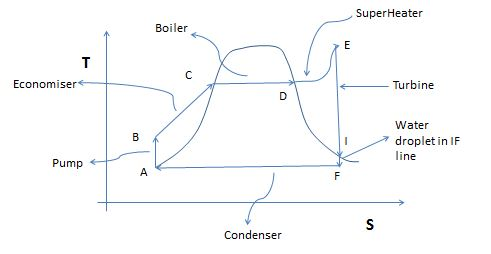
\includegraphics[width=0.6\textwidth]{captures/Capture2.JPG}
\caption{Thermal-Entropy Diagram for Water}
\end{figure}
\par Let us start our cycle from the boiler, i.e., the point $C$. From here, water is heated at constant temperature ($CD$ line) so that it becomes steam out of the boiler. Now, if the steam is extracted from the boiler (because it is needed to be extracted so that it is passed to turbine), it would again become water and so it is further heated to prevent this from happening by using a machine called superheater ($DE$ line). This superheat is restricted by a maximum temperature that is marked by point $E$ on the $T-S$ curve.  The superheated steam is passed to the turbine. A turbine ideally does not lose heat while extracting energy from superheated steam and so $dQ = 0 \implies dS = 0$, i.e., the entropy is constant but the temperature falls down until it again starts to condense to water ($EF$ line), but not much else it would corrode the material of turbine. It is allowed to form some water droplets. Now energy is extracted by the turbine which moves a generator coil to generate electricity.

\par Now, after the turbine has extracted the energy, the condenser takes out the heat from the incoming steam at constant temperature, hence entropy falls at constant temperature and the steam comes out as water ($FA$ line). Pump requires less energy to operate because it works on water, a low temperature form of steam. So like turbine it must also have constant entropy. But since you are pushing water, there is some work happening and therefore a rise in temperature ($AB$ line). Now boiler is at temperature beyond $100^{o}$ Celsius and the water out of the pump is at low temperature, hence if directly pushed to the boiler, the incoming water may produce a thermal stress in it and may crack it as well.  Therefore a new device called the economizer brings temperature of water close to 100 ($BC$ line). $S$ is decreased and $T$ is increased and the $T-S$ cycle is completed.

\subsection{Actual power plant for implementing the $T-S$ diagram}
\par In most modern thermal power plants, coal is {\it pulverized} into powder and then blown with air inside the chimney so that complete combustion takes place. The structure of the column (chimney) is such that there are two ports inserting the pulverized coal into the column in vertically slant direction so that a vortex is created and it is continuously churned to prevent its settlements on the ground. The gases rise in the column after burning. Some burned part of coal settles down and some goes up with gas. At top of the column, there is a boiler drum. The drum stores the water. The water comes out of the boiler through pipes along side the walls of the columns from outside which are at high temperatures and inserted into the column through a port which is at the lowermost point of the column. There are pipes inside also of the column which take the water from that port back up to the boiler again. The actual steam conversion happens in the inner pipes. There are many such pipes. So there is a circulation of water in pipes and the water is converted to steam. In fact, there are so many pipes inside, that the flame inside the column never sees the actual walls. These collection of pipes is called the {\it water walls}. Steam is formed above the water inside the boiler drum which has to be taken out. Now this is to be further heated so that it does not become water back, a work that has to be done by the superheater.

\par The flue gas that is rising inside the column is still at a high temperature and the steam is circulated in that gas. The superheater is this only. The output is a superheated steam. Now this steam is sent to the turbine.  The turbine is in a shape of trapezoid so that the shorter side is given to the incoming high pressure steam and the outgoing steam is given the longer side so that it can expand easily. High pressure steam is converted to low pressure steam. So there are generally 3 turbines, one high pressure turbine, one intermediate pressure turbine and a low pressure turbine. 
\\ 
\begin{figure}[H]
\centering 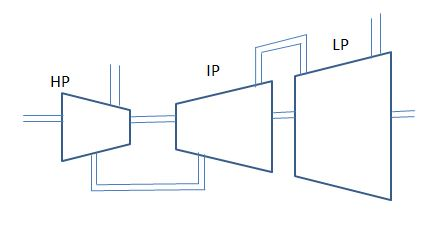
\includegraphics[width=0.6\textwidth]{captures/Capture4.JPG}
\caption{Turbines in a power plant}
\end{figure}
\par Therefore, the pressure of steam is reduced in steps. Next the low pressure steam goes to a condenser. In condenser there is an inlet for cold water which condenses the steam and the cold water becomes hot as a byproduct. The output is condensed steam. This cold water comes from the water bodies. This hot water is cooled down naturally before throwing it back to the environment, using cooling towers where cool air is used to cool the water. This takes in a lot of heat from the hot water. 
The efficiency of a thermodynamic process is given by
\begin{equation}
\displaystyle \eta_{eff} = 1 - \frac{T_{sink}}{T_{source}}
\end{equation}
Where $T$ is the temperature in $K$. Here, sink temperature is the temperature inside the condenser, say, 303 K. Source temperature is the temperature to which the superheater heats up the steam, say 673 K. Thus, the efficiency is  approximately 50 \%. Actual efficiency if 35 to 38 \% in practical systems. Because of this low efficiency, a great deal of heat has to be released to the atmosphere. This is a source of thermal pollution. 

\par The condensed heat is fed to economizer, which increases the temperature of steam water close to 100 and feds it back to the boiler drum. As an Engineer, it is our duty to increase this efficiency so that the hot water released from the condenser is not at such a high temperature (reducing thermal pollution). That is the power extracted from the condenser is the area under $ABCA$ in the $T-S$ curve. We need to increase this area. For that we need to bring the $FA$ line to even more lower level (condenser line). This means increasing the length of $EF$ line or in other words,  more expansion of steam must be done by the turbine. This has a negative effect. This will make water droplets to rise and that will corrode the turbine. Thus, this cannot be done. Now one would suggest that if that cannot be done, lets increase the level of $CD$ line in the $T-S$ plot, that would mean to increase the temperature in boiler and thus high pressure in boiler. That may explode the boiler drum.  This limit can however be overcome if we threw away the boiler drum concept. Thus we fail here also. We could increase the pump energy to increase that area. Pumping energy is provided by us. This is an option but then the overall efficiency of electricity generation will be lowered because we are already producing electricity over here.

\par What is actually done is, at some point $G$, after high pressure stage turbine, the steam is extracted and again allowed to expand so that it reaches the point $H$ (which is at lower temperature than $E$) and the area is increased ($ar. JCKJ > ar. ABCA$). The new $T-S$ curve looks like this. The device that heats it again is called a reheater and then it is allowed to go to the intermediate pressure turbine. In this way we can increase the efficiency of the process.
\\ 
\begin{figure}[H]
\centering 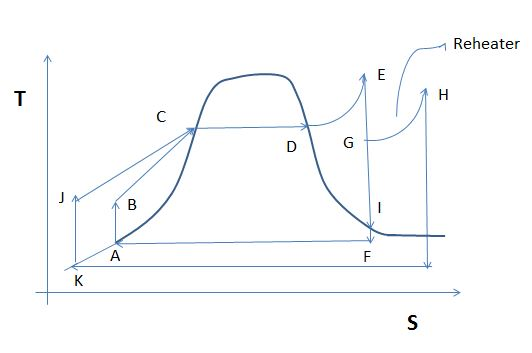
\includegraphics[width=0.6\textwidth]{captures/Capture3.JPG}
\caption{T-S Curve}
\end{figure}

\begin{thebibliography}{999}
\bibitem{lambport}
https://www.youtube.com/watch?v=8uwrMLrqQlU
\bibitem{lambport}
http://www.thermodyneboilers.com/components-working-thermal-power-plant/
\bibitem{lambport}
https://en.wikipedia.org/wiki/File:PowerStation2.svg
\end{thebibliography}
\end{document}